\chapter{光合作用和气孔导度}
%\addcontentsline{toc}{chapter}{光合作用和气孔导度}
\begin{mymdframed}{代码}
本节对应的代码文件为\texttt{MOD\_AssimStomataConductance.F90}。
\end{mymdframed}

%\begin{光合作用和气孔导度}

\section{植物的光合作用}\label{植物的光合作用}
CoLM光合作用模型是建立在冠层尺度,双大叶冠层结构基础上的。即冠层尺度的光合同化速率($A_{n}$)等于阳叶冠层的光合同化速率($A_{n,sun}$)加上阴叶冠层的光合同化速率($A_{n,sun}$):
\begin{equation}\label{Ansun_Ansha}
A_{n}=A_{n,sun}+A_{n,sha}
\end{equation}

阳叶和阴叶冠层尺度的光合同化速率模拟是通过对叶片尺度的光合作用模型进行升尺度而得到。C3植物叶片尺度的光合作用模拟是基于Farquhar光合作用模型~\citep{farquhar1980biochemical},
C4植物则是基于~\citet{collatz1992} 的光合作用改进模型。卡尔文循环是高等植物光合作用中的重要途径之一,CO$_2$和1,5-二磷酸核酮糖(RuBP)在1,5-二磷酸核酮糖羧化酶(Rubisco)的催化下产生羧化反应,生成3-磷酸甘油酸(PGA),并被还原为3-磷酸甘油醛(PGAL),PGA经过一系列转变再次形成RuBP,这被称为RuBP的再生阶段,完成卡尔文循环。当RuBP充足,卡尔文循环稳定时,多余的PGAL才会合成蔗糖和淀粉作为光合作用的产物存储在植物内。Faquhar模型认为卡尔文循环中的羧化速率($A_{c}$)和RuBP的再生速率是限制($A_{j}$)是光合作用总速率的两个关键限制因子,CoLM光合作用模块在此基础上增加了蔗糖和淀粉产物合成的速率限制($A_{p}$)。另外,叶片净光合同化速率 ($A_{n}$) 等于总光合同化速率减去叶呼吸速率 ($R_d$),在阴叶和阳叶冠层分别有:
\begin{equation}\label{An1sun}
A_{n,sun}=\min \left(A_{c,sun}, A_{j,sun}, A_{p,sun}\right)-R_{d,sun}
\end{equation}
\begin{equation}\label{An1sha}
A_{n,sha}=\min \left(A_{c,sha}, A_{j,sha}, A_{p,sha}\right)-R_{d,sha}
\end{equation}
其中,下标$sun$和$sha$分别代表在阳叶和阴叶冠层尺度上的光合同化速率和呼吸速率。


RuBP羧化酶限制主要指当羧化酶活性较低时,光合作用羧化速率受限,也称为Rubisco限制。由于Rubisco同时催化RuBP的羧化反应和氧化反应,羧化反应需要CO$_2$而氧化反应需要O$_2$,羧化反应和氧化反应同时进行。因此,C3植物的胞间CO$_2$分压$c_i$和O$_2$分压$o_i$的比例极大影响了Rubisco作为羧化酶的效率。基于这个原因,C3植物的Rubisco限制下的光合同化速率($A_c$)可表达为Michaelis-Menten关于$c_i$和$o_i$的函数。此外,C4植物Rubisco限制下的光合羧化速率不再受胞间CO$_2$分压和O$_2$分压的影响,这是由于C4植物的光合作用途径的最初步骤是PEP的羧化,PEP羧化酶的活性很高,所以转运到维管束鞘细胞中的CO$_2$的浓度很高,大约是空气中的十倍。C4植物的卡尔文循环在在维管束鞘细胞进行,CO$_2$分压和O$_2$分压的变化对羧化速率的影响较小,因此,Rubisco限制下的光合同化速率在阳叶和阴叶冠层尺度($A_{c,sun}$和$A_{c,sha}$)下可表示为胞间CO$_2$分压($c_{i,sun}$和$c_{i,sha}$),大气分压($o_{i}$)和最大羧化速率的函数($V_{c \max,sun}$和$V_{c \max,sha}$):
\begin{equation}\label{A_C1sun}
A_{c,sun}=\begin{cases}
\frac{V_{c \max,sun}\left(c_{i,sun}-\Gamma_{sun}\right)}{c_{i,sun}+K_{c}\left(1+\frac{o_{i}}{K_{o}}\right)}
     & \text{for C3 plants} \\ 
V_{c \max,sun } & \text{for C4 plants}
\end{cases}
\end{equation}
\begin{equation}\label{A_C1sha}
A_{c,sha}=\begin{cases}
\frac{V_{c \max,sha}\left(c_{i,sha}-\Gamma_{sha}\right)}{c_{i,sha}+K_{c}\left(1+\frac{o_{i}}{K_{o}}\right)}
     & \text{for C3 plants} \\ 
V_{c \max,sha } & \text{for C4 plants}
\end{cases}
\end{equation}

其中,下标$sun$和$sha$分别代表在阳叶和阴叶冠层尺度上的相应变量,$\Gamma$是CO$_2$补偿点,$K_c$和$K_o$分别是对于CO$_2$和O$_2$的Michaelis--Menten常数(Pa),$V_{c \max,sun}$和$V_{c \max,sha}$代表阳叶和阴叶冠层尺度的最大羧化速率,它是根据叶面积指数从叶片尺度上升到冠层尺度的光合参数。

C3植物:
\begin{equation}\label{V_cmaxsun_a}
V_{c \max,sun }=\frac{V_{c \max 25} \cdot 2.1^{\frac{T_{{leaf }}-T_{o p}}{10}}}{1+e^{s_{1}\left(T_{{leaf }}-T_{{high }}\right)}} \cdot \beta_{sun} \cdot L_{v,sun}
\end{equation}
\begin{equation}\label{V_cmaxsha_a}
V_{c \max,sha }=\frac{V_{c \max 25} \cdot 2.1^{\frac{T_{{leaf }}-T_{o p}}{10}}}{1+e^{s_{1}\left(T_{{leaf }}-T_{{high }}\right)}} \cdot \beta_{sha} \cdot L_{v,sha}
\end{equation}

C4植物:
\begin{equation}\label{V_cmaxsun_b}
V_{c \max,sun }= \frac{V_{c \max 25} \cdot 2.1^{\frac{T_{{leaf }}-T_{o p}}{10}}}{\left(1+e^{s_{2}\left(T_{{low }}
 - T_{{leaf }}\right)}\right)\left(1+e^{s_{1}\left(T_{{leaf }}-T_{h i g h}\right)}\right)} \cdot \beta_{sun} \cdot L_{v,sun}
\end{equation}
\begin{equation}\label{V_cmaxsha_b}
V_{c \max,sha }= \frac{V_{c \max 25} \cdot 2.1^{\frac{T_{{leaf }}-T_{o p}}{10}}}{\left(1+e^{s_{2}\left(T_{{low }}
 - T_{{leaf }}\right)}\right)\left(1+e^{s_{1}\left(T_{{leaf }}-T_{h i g h}\right)}\right)} \cdot \beta_{sha} \cdot L_{v,sha}
\end{equation}
不同植被的羧化能力存在差异,我们用25 \textcelsius 下的最大羧化速率 $V_{c \max 25}$ 来刻画植被的光合羧化能力,单位: \unit{mol.m^{-2}.s^{-1}};Rubisco羧化酶的活性随温度显著变化,CoLM光合作用模块针对C3和C4植物制定了两套温度响应函数。$T_{op}$是参考温度298 K;$s_1$和$s_2$分别为高温和低温的温度敏感性参数;$T_{low}$和$T_{high}$分别为羧化速率的低温和高温响应参数,
取值根据植被类型而变化,范围分别为: 278$\sim$288 K,303$\sim$313 K;$T_{leaf}$是叶片温度,通过对叶片能量平衡方程进行牛顿迭代方法而求解得到,详见章节~\ref{植被叶片温度计算},$\beta_{sun}$和$\beta_{sha}$是阳叶和阴叶的水分胁迫因子,水分胁迫因子的取值范围0$\sim$1,详见章节~\ref{气孔导度的水分胁迫}。当植被水力模式开启时,需要最大气孔导度作为植被水力模式输入,在水分胁迫因子为1的条件下,光合气孔耦合模型可得到最大气孔导度。另外,$L$代表叶片到冠层的尺度转换系数,下标sun和sha分别代表阳叶和阴叶,$v$代表参数$V_{c \max}$的转换系数,它们均是叶面积指数的函数:
%
\begin{equation}\label{L_vsun}
L_{v,sun}=\frac{1-e^{-\left(0.11+K_{b}\right) \cdot LAI}}{0.11+K_{b}}
\end{equation}
\begin{equation}\label{L_vsha}
L_{v,sha}=\frac{1-e^{-0.11\cdot LAI}}{0.11} - L_{v,sun}
\end{equation}
$K_{b}$代表直射光的消光系数。

当光照不足时,RuBP再生速率下降,成为制约光合作用开尔文循环的最主要因素。因此,RuBP再生速率限制下的羧化速率在阳叶和阴叶冠层尺度下 ($A_{j,sun}$和$A_{j,sha}$) 可表达为阳叶和阴叶的有效光合辐射 ($PAR_{sun}$和$PAR_{sha}$) 的函数:
\begin{equation}\label{A_J1sun}
A_{j,sun}=\begin{cases}\frac{J_{x,sun}\cdot\left(c_{i,sun}-\Gamma\right)}{4c_{i,sun}+8\Gamma}
     & \text{for C3 plants} \\
\alpha\left(4.6 \times 10^{-6} \cdot PAR_{sun}\right) & \text{for C4 plants}
\end{cases}
\end{equation}
\begin{equation}\label{A_J1sha}
A_{j,sha}=\begin{cases}\frac{J_{x,sha}\cdot\left(c_{i,sha}-\Gamma\right)}{4c_{i,sha}+8\Gamma}
     & \text{for C3 plants} \\
\alpha\left(4.6 \times 10^{-6} \cdot PAR_{sha}\right) & \text{for C4 plants}
\end{cases}
\end{equation}

$J_{x,sun}$和$J_{x,sha}$是阳叶和阴叶冠层尺度的电子传输速率,是有效光合辐射($PAR_{sun}$和$PAR_{sha}$)的函数,并受叶片温度 ($T_{leaf}$)和水分胁迫因子($\beta_{sun}$和$\beta_{sha}$)的调节:
\begin{equation}
\begin{aligned}
J_{x,sun}=\min \left(\begin{array}{c} \alpha\left(4.6 \times 10^{-6} \cdot PAR_{sun}\right), \\
  J_{x25} \cdot \exp\left(\frac{37000\left(T_{{leaf }}-T_{o p}\right)\left[1+\exp\left(\frac{710 \cdot T_{o p}-220000}
 {R \cdot T_{o p}}\right)\right]R \cdot T_{{leaf}}}{T_{o p} \cdot T_{{leaf }} \cdot R 
 \cdot \left(710 \cdot T_{{leaf }}-220000\right)}\right)\cdot \beta_{sun} \cdot L_{j,sun}  \end{array} \right)  
\end{aligned}
\end{equation}
\begin{equation}
\begin{aligned}
J_{x,sha}=\min \left(\begin{array}{c} \alpha\left(4.6 \times 10^{-6} \cdot PAR_{sha}\right), \\
  J_{x25} \cdot \exp\left(\frac{37000\left(T_{{leaf }}-T_{o p}\right)\left[1+\exp\left(\frac{710 \cdot T_{o p}-220000}
 {R \cdot T_{o p}}\right)\right]R \cdot T_{{leaf}}}{T_{o p} \cdot T_{{leaf }} \cdot R 
 \cdot \left(710 \cdot T_{{leaf }}-220000\right)}\right)\cdot \beta_{sha} \cdot L_{j,sha}  \end{array} \right)  
\end{aligned}
\end{equation}
其中$\alpha$是量子效率 (\qty{0.05}{mol.CO_2.mol^{-1}.photon});$PAR$是有效光合辐射,单位: \unit{W.m^{-2}},详细计算见章节~\ref{短波吸收辐射通量};
\num{4.6e-6} 代表单位从 \unit{W.m^{-2}} 转换到 \unit{mol.photon.m^{-2}} 的转换系数;
$J_{x25}$是25 \textcelsius 下的最大电子传输速率,单位: \unit{mol.m^{-2}.s^{-1}},$J_{x25}=1.97 \cdot V_{c \max 25}$; 
$R$是通用气体常数,$R=$ \qty{8.3145}{mol.m^{-2}.s^{-1}}。$L_{j,sun}$和$L_{j,sha}$代表电子传输速率的尺度转换系数(叶片到冠层):
%
\begin{equation}\label{L_jsun}
L_{j,sun}=\frac{1-e^{-\left(K_{d}+K_{b}\right) \cdot LAI}}{K_{d}+K_{b}}
\end{equation}
\begin{equation}\label{L_jsha}
L_{j,sha}=\frac{1-e^{-K_{d}\cdot LAI}}{K_{d}} - L_{j,sun}
\end{equation}
$K_{d}$代表散射光的消光系数。

第三,光合作用速率还受到卡尔文循环中蔗糖和淀粉的合成速率限制($A_{p,sun}$和$A_{p,sha}$),在阳叶和阴叶冠层尺度上,用冠层25 \textcelsius 最大羧化速率 ($V_{c \max25}$) 进行参数化,并且描述其受叶温和水分胁迫因子的调控:

C3植物:
\begin{equation}\label{A_e_a_sun}
A_{p,sun}=\frac{V_{c \max 25}}{2} \cdot \frac{1.8^{\frac{T_{{leaf }}-T_{o p}}{10}}}{1+e^{s_{2}\left(T_{{low }}-T_{{leaf }}\right)}} \cdot \beta_{sun} \cdot L_{v,sun}
\end{equation}
\begin{equation}\label{A_e_a_sha}
A_{p,sha}=\frac{V_{c \max 25}}{2} \cdot \frac{1.8^{\frac{T_{{leaf }}-T_{o p}}{10}}}{1+e^{s_{2}\left(T_{{low }}-T_{{leaf }}\right)}} \cdot \beta_{sha} \cdot L_{v,sha}
\end{equation}

C4植物:
\begin{equation}\label{A_e_b_sun}
A_{p,sun}=\frac{V_{c \max 25}}{5} \cdot 1.8^{\frac{T_{{leaf }}-298.16}{10}} \cdot \beta_{sun} \cdot L_{v,sun}
\end{equation}
\begin{equation}\label{A_e_b_sha}
A_{p,sha}=\frac{V_{c \max 25}}{5} \cdot 1.8^{\frac{T_{{leaf }}-298.16}{10}} \cdot \beta_{sha} \cdot L_{v,sha}
\end{equation}
三方面限制下的光合同化速率共用同一套温度响应常数 ($T_{op}$,$T_{low}$和$T_{high}$)以及温度敏感性参数($s_1$和$s_2$)


阳叶和阴叶冠层尺度的呼吸速率($R_{d,sun}$和$R_{d,sha}$)对温度的响应曲线可表示为$V_{c \max25}$的函数:
\begin{equation}\label{R_d1_sun}
R_{d,sun}=r_{{base }} \cdot V_{cmax 25} \cdot \frac{2.0^{\frac{T_{leaf}-T_{op}}{10}}}{1+e^{1.3 \cdot\left(T_{leaf}-T_{d m}\right)}} \cdot \beta_{sun} \cdot L_{v,sun}
\end{equation}
\begin{equation}\label{R_d1_sha}
R_{d,sha}=\tau_{{base }} \cdot V_{cmax 25} \cdot \frac{2.0^{\frac{T_{leaf}-T_{op}}{10}}}{1+e^{1.3 \cdot\left(T_{leaf}-T_{d m}\right)}} \cdot \beta_{sha} \cdot L_{v,sha}
\end{equation}
其中$T_{dm}$是叶呼吸的高温抑制温度常数,单位 K; $\tau_{base}$是基础呼吸速率系数,无量纲。

在方程\eqref{An1sun}和\eqref{An1sha}求解最小值的计算中,我们将三值最小问题的求解拆分为两个二值最小问题的求解:
\begin{equation}\label{min_Ac_Aj_Ae}
\min \left(A_{c}, A_{j}, A_{e}\right)=\min \left(\min \left(A_{c}, A_{j}\right), A_{e}\right)
\end{equation}
引入形状参数$\theta$,构造一元二次方程,将求解最小值问题转换成求一元二次方程较小根的问题,以此避免模拟中不同光合限制之间过渡转换时的光合同化速率突变 \citep{collatz1991,collatz1992}:
\begin{equation}\label{theta_cj}
\theta_{c j} \cdot A_{i1}^{2}-\left(A_{c}+A_{j}\right) A_{i1}+A_{c} A_{j}=0
\end{equation}
\begin{equation}\label{theta_cje}
\theta_{c j e} \cdot A_{i2}^{2}-\left(A_{i1}+A_{e}\right) A_{i2}+A_{i1} A_{e}=0
\end{equation}
其中形状参数$\theta_{cj}=0.877$,$\theta_{cje}=0.95$。$A_{i1}$为方程\eqref{theta_cj}的较小根,代表$A_c$和$A_j$的最小值。$A_{i2}$为方程\eqref{theta_cje}的较小根,代表$A_{i1}$和$A_e$的最小值。


\section{气体扩散方程和气孔导度模型}\label{气体扩散方程和气孔导度模型}
气孔是植被和大气相互作用的最重要通道,陆地生态系统碳水耦合很大程度取决于气孔的行为。CoLM在的光合同化速率和蒸腾速率计算中,考虑植被气孔的行为,结合气体扩散方程,刻画了碳水通量与浓度梯度之间的重要关系~\eqref{A_n2_sun}--\eqref{ea_ei_sha}。CoLM将CO$_2$和水汽的气体扩散问题类比于电路问题进行建模,利用叶绿体细胞间、叶表和冠层大气的$\rm CO_2$浓度和水汽浓度梯度,来刻画环境对植被碳水通量的驱动力,如图~\ref{fig:叶片气孔光合作用导度模型示意图}。因此,在阳叶和阴叶冠层尺度上,分别存在关于$\rm CO_2$和水汽的气体扩散方程:

{
\begin{figure}[htbp]
\centering
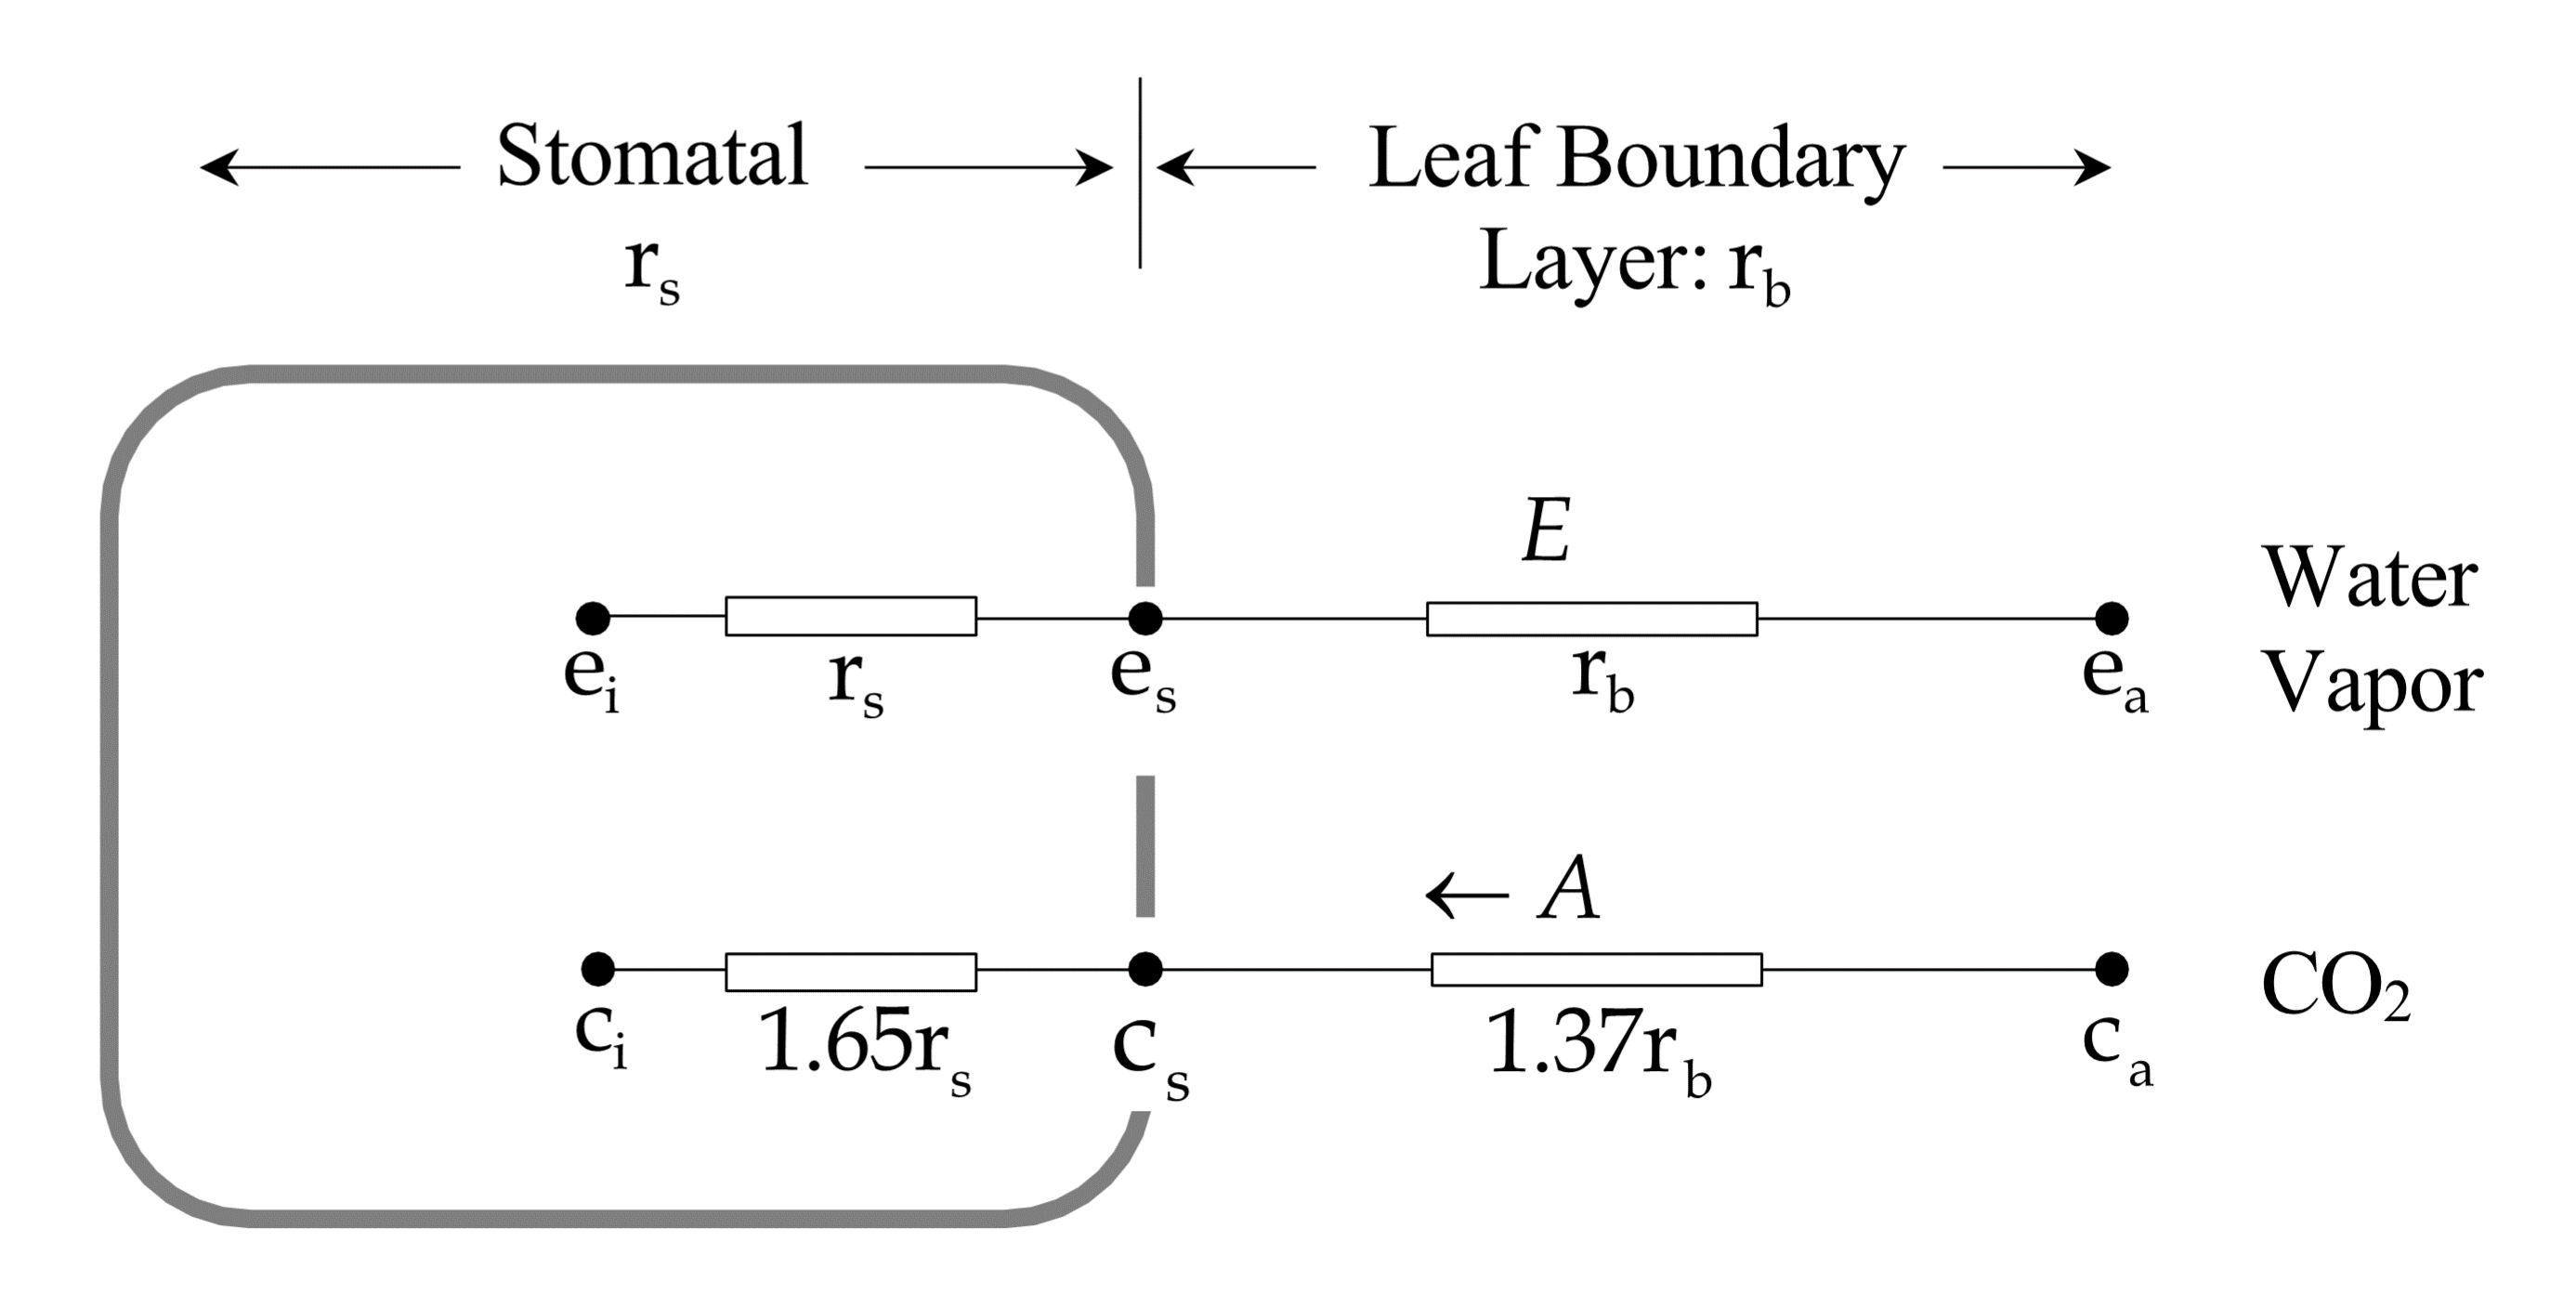
\includegraphics[width=0.8\textwidth]{Figures/气孔导度和光合作用/叶片气孔光合作用导度模型示意图.png}
\caption{叶片气孔光合作用导度模型示意图}
\label{fig:叶片气孔光合作用导度模型示意图}
\end{figure}
}

\begin{equation}\label{A_n2_sun}
A_{n,sun}=\left(c_{a}-c_{s,sun}\right) /\left(\frac{1.37}{G_{b}} p_{s}\right)=\left(c_{s,sun}-c_{i,sun}\right) /\left(\frac{1.6}{G_{s,sun}} p_{s}\right)
\end{equation}
\begin{equation}\label{A_n2_sha}
A_{n,sha}=\left(c_{a}-c_{s,sha}\right) /\left(\frac{1.37}{G_{b}} p_{s}\right)=\left(c_{s,sha}-c_{i,sha}\right) /\left(\frac{1.6}{G_{s,sha}} p_{s}\right)
\end{equation}
\begin{equation}\label{ea_ei_sun}
\left(e_{a}-e_{i}\right) /\left(\frac{1}{G_{b}}+\frac{1}{G_{s,sun}}\right)=\left(e_{s,sun}-e_{i}\right) / \frac{1}{G_{s,sun}}
\end{equation}
\begin{equation}\label{ea_ei_sha}
\left(e_{a}-e_{i}\right) /\left(\frac{1}{G_{b}}+\frac{1}{G_{s,sha}}\right)=\left(e_{s,sha}-e_{i}\right) / \frac{1}{G_{s,sha}}
\end{equation}
其中,$c_{i,sun}$和$c_{i,sha}$是阳叶和阴叶的胞间CO$_2$分压,$c_{s,sun}$和$c_{s,sha}$是阳叶和阴叶的叶表CO$_2$分压,$c_a$是冠层大气$\rm CO_2$分压,叶表水汽分压$e_{s,sun}$和$e_{s,sha}$,$e_a$是冠层大气水汽分压,$e_i$是胞间水汽分压,单位: Pa,通常假定为饱和水汽压,$G_b$是冠层尺度的叶边界层导度,$G_{s,sun}$和$G_{s,sha}$是阳叶和阴叶的冠层尺度叶气孔导度,单位: \unit{mol.m^{-2}.s^{-1}};单位: Pa。

气孔导度理论认为植被根据自身光合同化速率、环境大气水分亏缺以及土壤水分胁迫等因素,主动调控气孔导度。CoLM的气孔导度计算沿用Ball-Berry模型,但将尺度从叶片扩展到冠层,Ball-Berry模型根据冠层净光合同化速率 
($A_n$,单位: \unit{mol.CO_2.m^{-2}.s^{-1}})、叶表水汽压 ($e_{s,sun}$和$e_{s,sha}$,单位: Pa)、叶表二氧化碳分压 ($c_{s,sha}$和$c_{s,sha}$,单位: Pa) 
基于气孔导度的观测回归经验关系,在阳叶和阴叶上分别计算冠层尺度的气孔导度 ($G_{s,sun}$和$G_{s,sha}$, 单位: \unit{mol.CO_2.m^{-2}.s^{-1}}): 
\begin{equation}\label{rs_a1sun}
\frac{1}{r_{s,sun}}=G_{s,sun}=m \frac{A_{n,sun}}{c_{s,sun}} \frac{e_{s,sun}}{e_{i}} p_{s}+b\beta_{sun}
\end{equation}
\begin{equation}\label{rs_a1sha}
\frac{1}{r_{s,sha}}=G_{s,sha}=m \frac{A_{n,sha}}{c_{s,sha}} \frac{e_{s,sha}}{e_{i}} p_{s}+b\beta_{sha}
\end{equation}
$r_{s,sun}$和$r_{s,sha}$代表阳叶和阴叶冠层尺度的气孔阻抗,单位: \unit{s.m^{-1}},是气孔导度$G_{s,sun}$和$G_{s,sha}$的倒数;$m$是无量纲经验参数;$b$是最小气孔导度,
单位: \unit{mol.CO_2.m^{-2}.s^{-1}},$m$和$b$是观测拟合的经验系数;$e_i$是饱和水蒸气压,
是气温的函数,单位: Pa;$p_s$是大气压强,单位: Pa,$\beta_{sun}$和$\beta_{sha}$是阳叶和阴叶的水分胁迫因子,取值范围0$\sim$1。


因为气孔控制植被大气气体交换的同时受植被自身的光合能力和土壤水分亏缺的影响,需要联立光合作用模块方程、气体扩散方程,气孔导度模型和土壤水分胁迫方案,在阳叶和阴叶上分别求解冠层尺度气孔导度。
由方程~\eqref{A_n2_sun}和~\eqref{A_n2_sha} 可知:
\begin{equation}\label{cs_a1sun}
c_{s,sun}=c_{a}-\frac{1.37 A_{n,sun}}{G_{b}} p_{s}
\end{equation}
\begin{equation}\label{cs_a1sha}
c_{s,sha}=c_{a}-\frac{1.37 A_{n,sha}}{G_{b}} p_{s}
\end{equation}
由方程~\eqref{ea_ei_sun}和~\eqref{ea_ei_sha}可知:
\begin{equation}\label{e_s1sun}
e_{s,sun}=\left(\frac{e_{a}}{G_{s,sun}}+\frac{e_{i}}{G_{b}}\right) /\left(\frac{1}{G_{b}}+\frac{1}{G_{s,sun}}\right)
\end{equation}
\begin{equation}\label{e_s1sha}
e_{s,sha}=\left(\frac{e_{a}}{G_{s,sha}}+\frac{e_{i}}{G_{b}}\right) /\left(\frac{1}{G_{b}}+\frac{1}{G_{s,sha}}\right)
\end{equation}
将方程~\eqref{e_s1sun}和~\eqref{e_s1sha}分别代入方程~\eqref{rs_a1sun}和~\eqref{rs_a1sha}中,得到关于$G_{s,sun}$和$G_{s,sha}$的两个一元二次方程:
\begin{equation}\label{ei_cssun}
\frac{e_{i} c_{s,sun}}{m A_{n,sun} p_{s}} G_{s,sun}^{2}+\left(\frac{e_{i} c_{s,sun}\left(G_{b} -b \beta_{sun}\right)}{m A_{n,sun} p_{s}}-e_{i}\right) G_{s,sun}
-e_{a} G_{b}+\frac{b \beta_{sun} G_{b} e_{i} c_{s,sun}}{m A_{n,sun} p_{s}}=0
\end{equation}
\begin{equation}\label{ei_cssha}
\frac{e_{i} c_{s,sha}}{m A_{n,sha} p_{s}} G_{s,sha}^{2}+\left(\frac{e_{i} c_{s,sha}\left(G_{b} -b \beta_{sha}\right)}{m A_{n,sha} p_{s}}-e_{i}\right) G_{s,sha}
-e_{a} G_{b}+\frac{b \beta_{sha} G_{b} e_{i} c_{s,sha}}{m A_{n,sha} p_{s}}=0
\end{equation}
冠层尺度的气孔导度 ($G_{s,sun}$和$G_{s,sha}$) 的解即为一元二次方程\eqref{ei_cssun}和\eqref{ei_cssha}的正根,其中叶片表层$\mathrm{CO_2}$分压 ($c_{s,sun}$和$c_{s,sha}$) 由方程~\eqref{cs_a1sun}和~\eqref{cs_a1sha} 得出,$A_{n,sun}$和$A_{n,sha}$由光合作用模块公式~\eqref{An1sun}和~\eqref{An1sha} 得出,
但仍然包含未知变量阳叶和阴叶的胞间 $\mathrm{CO_2}$ 分压 ($c_{i,sun}$和$c_{i,sha}$),完整求解光合气孔模式还需根据$\mathrm{CO_2}$气体扩散方程~\eqref{A_n2_sun}和~\eqref{A_n2_sha} 得出:
\begin{equation}\label{ci_1sun}
c_{i,sun}=c_{s,sun}-\frac{1.6 A_{n,sun} p_{s}}{G_{s,sun}}
\end{equation}
\begin{equation}\label{ci_1sha}
c_{i,sha}=c_{s,sha}-\frac{1.6 A_{n,sha} p_{s}}{G_{s,sha}}
\end{equation}
气孔导度-光合作用耦合问题可以被数学地抽象为求解非线性方程组问题,即联立方程~\eqref{An1sun}, ~\eqref{An1sha}, \eqref{cs_a1sun}, \eqref{cs_a1sha}, \eqref{ei_cssun}--%
%, \eqref{ei_cssha}, \eqref{ci_1sun}和
\eqref{ci_1sha},求解未知变量 $G_{s,sun}$, $G_{s,sha}$, $c_{i,sun}$, $c_{i,sha}$, $c_{s,sun}$, $c_{s,sha}$, $A_{n,sun}$和 $A_{n,sha}$。详细求解方案见章节~\ref{光合气孔耦合模型的数值计算方案}。


\section{光合气孔耦合模型的数值计算方案}\label{光合气孔耦合模型的数值计算方案}
由于光合作用Farquhar模型的非线性,且同时需要联立气体扩散方程和气孔导度方程,CoLM采用割线法和抛物线法的混合方法对气孔导度-光合作用耦合问题进行数值求解。上一节已经介绍过关于气孔导度--光合作用耦合问题需联立求解的8个方程~\eqref{An1sun}, \eqref{An1sha}, \eqref{cs_a1sun}, \eqref{cs_a1sha}, \eqref{ei_cssun}--%
%, \eqref{ei_cssha}, \eqref{ci_1sun}和
\eqref{ci_1sha}。其中,胞间$\mathrm{CO_2}$浓度是连接气孔导度模型和光合作用模型的关键,胞间$\mathrm{CO_2}$浓度既是Farquhar光合作用模型的输入,即方程~\eqref{An1sun}和~\eqref{An1sha}的自变量,又是气体扩散方程的输入,即方程~\eqref{cs_a1sun}, \eqref{cs_a1sha}, \eqref{ci_1sun} 和~\eqref{ci_1sha} 的自变量。同时,胞间$\mathrm{CO_2}$浓度($c_{s,sun}$)和叶表$\mathrm{CO_2}$浓度$c_{s,sha}$)之间的浓度梯度也是刻画光合同化速率($A_{n,sun}$和$A_{n,sha}$)和气孔导度关系的重要变量。因此原方程组可简化为两个零点方程$f_1(c_{i,sun})=0$和$f_2(c_{i,sha})=0$。方程组的求解问题可等价为对目标函数$f_1(c_{i,sun})$和$f_2(c_{i,sha})$的零点搜索问题,具体目标函数可化为:
\begin{align}\label{f1_cisun}
f_{1}\left(c_{i,sun}\right)=&\,c_{i,sun}-c_{s,sun}\big(A_{n,sun}\left(c_{i,sun}\right)\big) \nonumber \\[1ex] 
+& \, \frac{1.6A_{n,sun}\left(c_{i,sun}\right)p_s}{G_{s,sun}\Big(A_{n,sun}\left(c_{i,sun}\right),c_{s,sun}\big(A_{n,sun}\left(c_{i,sun}\right)\big)\Big)}
\end{align}
\begin{align}\label{f1_cisha}
f_{2}\left(c_{i,sha}\right)=&\,c_{i,sha}-c_{s,sha}\big(A_{n,sha}\left(c_{i,sha}\right)\big) \nonumber \\[1ex] 
+& \, \frac{1.6A_{n,sha}\left(c_{i,sha}\right)p_s}{G_{s,sha}\Big(A_{n,sha}\left(c_{i,sha}\right),c_{s,sha}\big(A_{n,sha}\left(c_{i,sha}\right)\big)\Big)}
\end{align}

{
\begin{figure}[htbp]
\centering
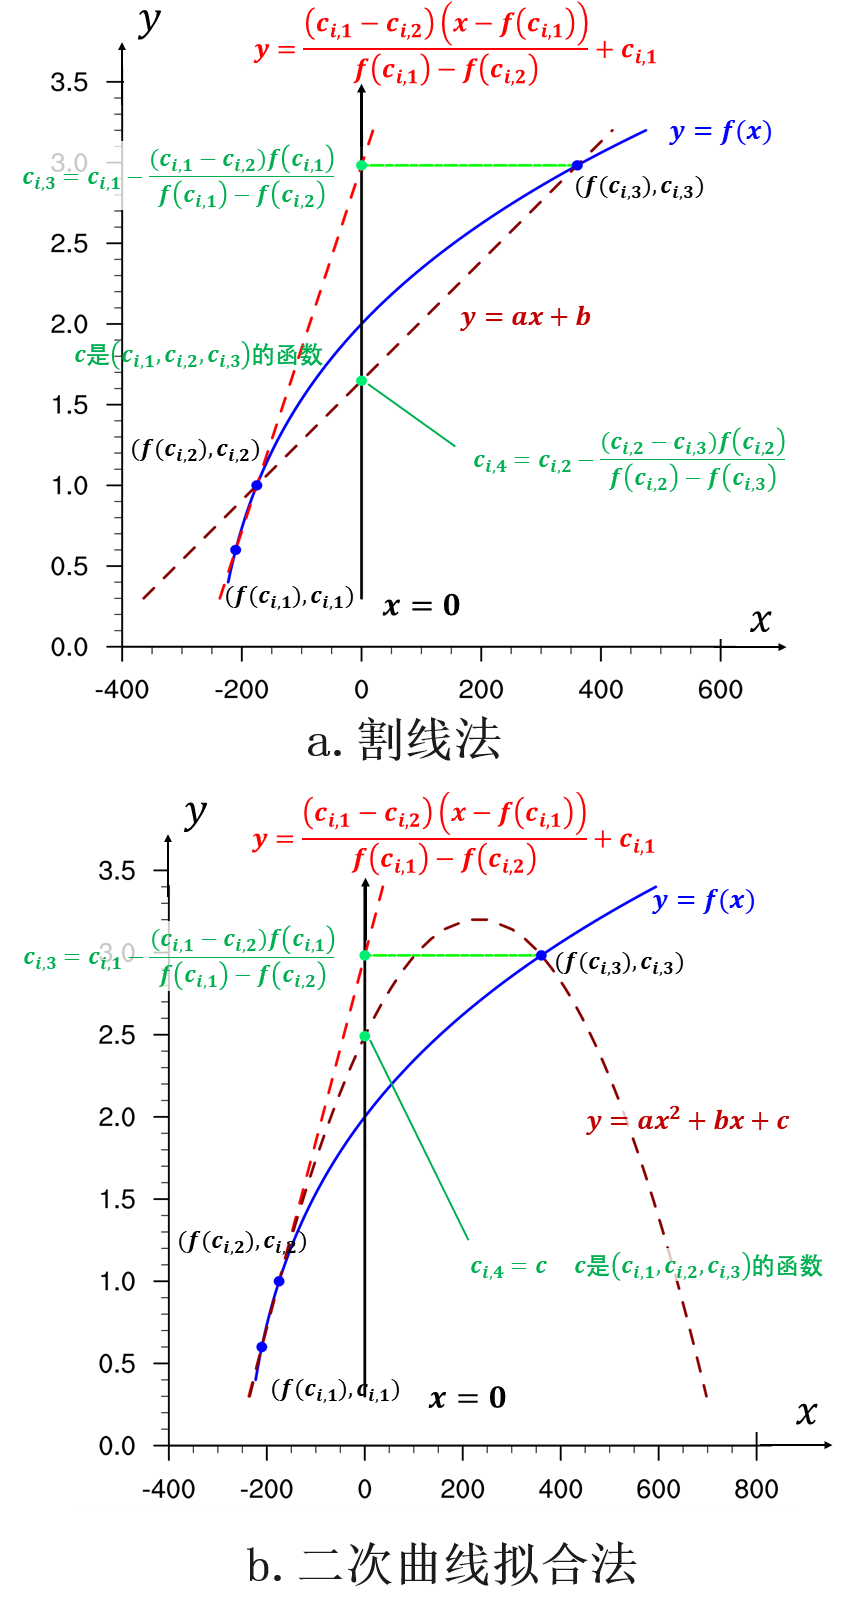
\includegraphics[width=0.56\textwidth]{Figures/气孔导度和光合作用/光合气孔耦合模型数值解法示意图.png}
\caption[光合气孔耦合模型数值解法示意图]{光合气孔耦合模型数值解法示意图,割线法对前两次迭代结果进行线性拟合,拟合结果和$x=0$的交点即为下一轮迭代的胞间$\rm CO_2$浓度的取值,拟合方程$y=ax+b$;二次方程拟合法对前三次迭代结果进行二次曲线拟合,拟合结果和$x=0$的交点即为下一轮迭代的胞间$\rm CO_2$浓度的取值,拟合方程$y=ax^2+bx+c$。

其中割线法的拟合方程系数为:

$\begin{cases}a=\frac{c_{i,n-1}-c_{i,n-2}}{f\left(c_{i,n-1}-c_{i,n-2}\right)}\\b=c_{i,n-2}-a\cdot f\left(c_{i,n-2}\right)\end{cases}$

二次方程拟合法的拟合方程系数为:

$\begin{cases}a=\frac{\left(c_{i,n-2}-c_{i,n-3}\right)-\left[f\left(c_{i,n-2}\right)-f\left(c_{i,n-3}\right)\right]b}{f^2\left(c_{i,n-2}\right)-f^2\left(c_{i,n-3}\right)}\\
b=\frac{\left(c_{i,n-2}-c_{i,n-3}\right)\left[f^2\left(c_{i,n-1}\right)-f^2\left(c_{i,n-2}\right)\right]-\left(c_{i,n-1}-c_{i,n-2}\right)\left[f^2\left(c_{i,n-2}\right)-f^2\left(c_{i,n-3}\right)\right]}{\left[f\left(c_{i,n-2}\right)-f\left(c_{i,n-3}\right)\right]\left[f^2\left(c_{i,n-1}\right)-f^2\left(c_{i,n-2}\right)\right]-\left[f\left(c_{i,n-1}\right)-f\left(c_{i,n-2}\right)\right]\left[f^2\left(c_{i,n-2}\right)-f^2\left(c_{i,n-3}\right)\right]}\\
c=c_{i,n-2}-af^2\left(c_{i,n-2}\right)-bf\left(c_{i,n-2}\right)\end{cases}$}
\label{fig:光合气孔耦合模型数值解法示意图}
\end{figure}
}

对目标函数的零点搜索过程中,我们采用割线法和二次方程拟合法,两种方法相结合的办法(如图~\ref{fig:光合气孔耦合模型数值解法示意图})。在割线法中,$c_{i,sun,se,n}$和$c_{i,sha,se,n}$是第$n$次迭代的胞间$\rm CO_2$浓度,存在与任意两次之前迭代结果(不妨设为第$k$次和第$l$次)的递推关系:
\begin{equation}\label{cisunn}
c_{i,sun,se,n}=c_{i,sun,se,k}-f_{1}\left(c_{i,sun,se,k}\right)\frac{c_{i,sun,se,k}-c_{i,sun,se,l}}{ f_{1}\left(c_{i,sun,se,k}\right)-f_{1}\left(c_{i,sun,se,l}\right)} 
\end{equation}
\begin{equation}\label{cishan}
c_{i,sha,se,n}=c_{i,sha,se,k}-f_{2}\left(c_{i,sha,se,k}\right)\frac{c_{i,sha,se,k}-c_{i,sha,se,l}}{ f_{2}\left(c_{i,sha,se,k}\right)-f_{2}\left(c_{i,sha,se,l}\right)} 
\end{equation}

在二次方程拟合法中,$c_{i,sun,qd,n}$和$c_{i,sha,qd,n}$是第$n$次迭代的胞间$\rm CO_2$浓度,可由任意三次之前迭代的结果(不妨设为第$k$次,第$l$次和第$m$次)推导而出:
\begin{equation}\label{cisunq}
c_{i,sun,qd,n} =c_{i,sun,qd,l} \\
  -a_{sun}\cdot f^2_{1}(c_{i,sun,qd,l}) - b_{sun}\cdot f_{1}(c_{i,sun,qd,l})
\end{equation}
\begin{equation}\label{cishaq}
c_{i,sha,qd,n} =c_{i,sha,qd,l} \\
  -a_{sha}\cdot f^2_{2}(c_{i,sha,qd,l}) - b_{sha}\cdot f_{2}(c_{i,sha,qd,l})
\end{equation}

其中$a_{sun}$,$a_{sha}$,$b_{sun}$和$b_{sha}$分别由前两次和前三次迭代结果递推而得:
\begin{equation}\label{iterbsun}
b_{sun} = \frac{\Delta c_{i,sun}\left(k,l\right)\Delta f^2_1\left(l,m\right)-\Delta c_{i,sun}(l,m) \Delta f^2_1\left(k,l\right)}{\Delta f^2_1\left(l,m\right) \Delta f_1 \left(k,l\right)-\Delta f^2_1\left(k,l\right)\Delta f_1 \left(l,m\right)}
\end{equation}
\begin{equation}\label{iterasun}
a_{sun} = \frac{\left(c_{i,sun,dq,k}-c_{i,sun,dq,l}\right)-\left[f_1(c_{i,sun,dq,k})-f_1(c_{i,sun,dq,l})\right]\cdot b_{sun}}{f^2_1(c_{i,sun,dq,k})-f^2_1(c_{i,sun,dq,l})}
\end{equation}
\begin{equation}\label{iterbsha}
b_{sha} = \frac{\Delta c_{i,sha}\left(k,l\right)\Delta f^2_2\left(l,m\right)-\Delta c_{i,sha}(l,m) \Delta f^2_2\left(k,l\right)}{\Delta f^2_2\left(l,m\right) \Delta f_2 \left(k,l\right)-\Delta f^2_2\left(k,l\right)\Delta f_2 \left(l,m\right)}
\end{equation}
\begin{equation}\label{iterasha}
a_{sha} = \frac{\left(c_{i,sha,dq,k}-c_{i,sha,dq,l}\right)-\left[f_1(c_{i,sha,dq,k})-f_1(c_{i,sha,dq,l})\right]\cdot b_{sha}}{f^2_1(c_{i,sha,dq,k})-f^2_1(c_{i,sha,dq,l})}
\end{equation}
$\Delta$ 用于表示之前第$p$次和第$q$次迭代结果之间的差值:
\begin{equation}
\Delta c_{i,sun}(p,q)\equiv c_{i,sun,qd,p} - c_{i,sun,qd,q} 
\end{equation}
\begin{equation}
\Delta c_{i,sha}(p,q)\equiv c_{i,sha,qd,p} - c_{i,sha,qd,q} 
\end{equation}
\begin{equation}
\Delta f_1 \left(p,q\right)\equiv f_1(c_{i,sun,qd,p})-f_1(c_{i,sun,qd,q})
\end{equation}
\begin{equation}
\Delta f_2 \left(p,q\right)\equiv f_2(c_{i,sha,qd,p})-f_2(c_{i,sha,qd,q})
\end{equation}
\begin{equation}
\Delta f^2_1 \left(p,q\right)\equiv f^2_1(c_{i,sun,qd,p})-f^2_1(c_{i,sun,qd,q})
\end{equation}
\begin{equation}
\Delta f^2_2 \left(p,q\right)\equiv f^2_2(c_{i,sha,qd,p})-f^2_2(c_{i,sha,qd,q})
\end{equation}
另外,$k$,$l$和$m$的选择见数值方案解法流程图 (图~\ref{fig:气孔数值解法流程图})。

对于割线法来说,因为要运用方程~\eqref{cisunn} 和~\eqref{cishan} 对胞间$\rm CO_2$浓度进行猜解,需要至少两次之前迭代的结果。所以,胞间$\rm CO_2$浓度的前两次初始迭代的取值($c_{i,sun,1}$,$c_{i,sha,1}$,$c_{i,sun,2}$和$c_{i,sha,2}$)需要预先给定;对于二次方程拟合方法来说,因为方程~\eqref{cisunq} 和~\eqref{cishaq} 需要三次之前迭代的结果进行拟合,前三次初始迭代的胞间$\rm CO_2$浓度的取值也需要预先给定。由于两种方法都需要至少两次初始迭代结果,我们令割线法和二次方程拟合法的前两次初始迭代的胞间$\rm CO_2$浓度取值一致。

胞间$\rm CO_2$浓度的第1个初始迭代取值($c_{i,sun,1}$和$c_{i,sha,1}$),按C3、C4植物类型被区分:
\begin{align}\label{ci_1}
\begin{cases}
c_{i,sun,1}=c_{i,sha,1}=\frac{0.25 \cdot o_{i}} {2600 \cdot 0.57 ^\frac{T_{{leaf }} -  T_{o p}}{10}} + 0.5\cdot c_{a}\cdot\left(1-\frac{1.6}{m}\right) &\rm for\,\, C3\\
c_{i,sun,1}=c_{i,sha,1}=0.5\cdot c_{a}\cdot\left(1-\frac{1.6}{m}\right)   &\rm for\,\, C4
\end{cases}
\end{align}

胞间$\rm CO_2$浓度的第2个初始迭代取值($c_{i,sun,2}$和$c_{i,sha,2}$),和C3、C4植物类型和第一次猜解结果$f_{1}\left(c_{i,sun,1}\right)$,$f_{2}\left(c_{i,sha,1}\right)$的符号有关,这是为了让目标函数尽量接近0点:

如果$f_{1}\left(c_{i,sun,1}\right)\geqslant 0$则阳叶胞间$\rm CO2$浓度的第二次迭代取值为:
\begin{align}\label{cisun_2_fp}
c_{i,sun,2}=
\begin{cases}
\frac{0.4 \cdot o_{i}} {2600 \cdot 0.57 ^\frac{T_{{leaf }} -  T_{o p}}{10}} + 0.2\cdot c_{a}\cdot\left(1-\frac{1.6}{m}\right)  &\rm for\,\, C3\\
0.2\cdot c_{a}\cdot\left(1-\frac{1.6}{m}\right) &\rm for\,\, C4
\end{cases}
\end{align}

如果$f_{2}\left(c_{i,sha,1}\right)\geqslant0$,则阴叶胞间$\rm CO2$浓度的第二次迭代取值为:
\begin{align}\label{cisha_2_fp}
c_{i,sha,2}=
\begin{cases}
\frac{0.4 \cdot o_{i}} {2600 \cdot 0.57 ^\frac{T_{{leaf }} -  T_{o p}}{10}} + 0.2\cdot c_{a}\cdot\left(1-\frac{1.6}{m}\right)  &\rm for\,\, C3\\
0.2\cdot c_{a}\cdot\left(1-\frac{1.6}{m}\right) &\rm for\,\, C4
\end{cases}
\end{align}

如果$f_{1}\left(c_{i,sun,1}\right)<0$,则阳叶胞间$\rm CO2$浓度的第二次迭代取值为:
\begin{align}\label{cisun_2_fn}
c_{i,sun,2}=
\begin{cases}
\frac{0.1 \cdot o_{i}} {2600 \cdot 0.57 ^\frac{T_{{leaf }} -  T_{o p}}{10}} + 0.8\cdot c_{a}\cdot\left(1-\frac{1.6}{m}\right)  &\rm for\,\, C3\\
0.8\cdot c_{a}\cdot\left(1-\frac{1.6}{m}\right) &\rm for\,\, C4
\end{cases}
\end{align}

如果$f_{2}\left(c_{i,sha,1}\right)<0$,则阴叶胞间$\rm CO2$浓度的第二次迭代取值为:
\begin{align}\label{cisha_2_fn}
c_{i,sha,2}=
\begin{cases}
\frac{0.1 \cdot o_{i}} {2600. \cdot 0.57 ^\frac{T_{{leaf }} -  T_{o p}}{10}} + 0.8\cdot c_{a}\cdot\left(1-\frac{1.6}{m}\right)  &\rm for\,\, C3\\
0.8\cdot c_{a}\cdot\left(1-\frac{1.6}{m}\right) &\rm for\,\, C4
\end{cases}
\end{align}

二次方程拟合法的第三次迭代胞间$\rm CO2$浓度取值由割线法,按方程~\eqref{cisunn} 和~\eqref{cishan}计算得到:
%
\begin{equation}\label{cisun3}
c_{i,sun,qd,3}=c_{i,sun,1}-f_{1}\left(c_{i,sun,1}\right)\frac{c_{i,sun,1}-c_{i,sun,2}}{ f_{1}\left(c_{i,sun,1}\right)-f_{1}\left(c_{i,sun,2}\right)} 
\end{equation}
\begin{equation}\label{cisha3}
c_{i,sha,qd,3}=c_{i,sha,1}-f_{2}\left(c_{i,sha,1}\right)\frac{c_{i,sha,1}-c_{i,sha,2}}{ f_{2}\left(c_{i,sha,1}\right)-f_{2}\left(c_{i,sha,2}\right)} 
\end{equation}

三次初始迭代以后,迭代所估计的每一步胞间$\rm CO_2$浓度$\left(c_{i,sun,k}和c_{i,sha,k}\right)$由割线法和二次方程拟合法的平均值共同确定:
\begin{equation}
c_{i,sun,k}=\frac{c_{i,sun,se,k}+c_{i,sun,qd,k}}{2}
\end{equation}
\begin{equation}
c_{i,sha,k}=\frac{c_{i,sha,se,k}+c_{i,sha,qd,k}}{2}
\end{equation}

光合气孔耦合模型求解迭代算法的总体流程如流程图\ref{fig:气孔数值解法流程图}所示,包含一下几个步骤和规则:
\begin{enumerate}
\item 
根据方程~\eqref{ci_1}--\eqref{cisha3},分别计算最初三次迭代的胞间$\rm CO_2$浓度;
\item 
根据方程~\eqref{f1_cisun} 和~\eqref{f1_cisha} 和胞间$\rm CO_2$浓度初始值,计算前三次初始迭代的目标函数$f_1\left(c_{i,sun,k}\right)$,$f_2\left(c_{i,sha,k}\right)$ $\left(k=1,2,3\right)$;
\item
记录已有迭代结果按目标函数值进行排序,并找到最接近零点的两次(割线法)或三次迭代结果(二次方程拟合法),计算下一迭代的胞间$\rm CO_2$浓度;
\item
根据胞间$\rm CO_2$浓度猜解,计算一迭代的目标函数。
\item
判断目标函数是否满足退出条件,如果目标函数的绝对值小于阈值0.1,则停止迭代,否则,重复步骤3--5。最终结果将保存最后一次迭代的各个状态。
\end{enumerate}
此外,步骤5的迭代退出判断不仅在步骤4之后进行,在初始迭代的目标函数计算之后同样需要判断退出条件。

{
\begin{figure}[htbp]
\centering
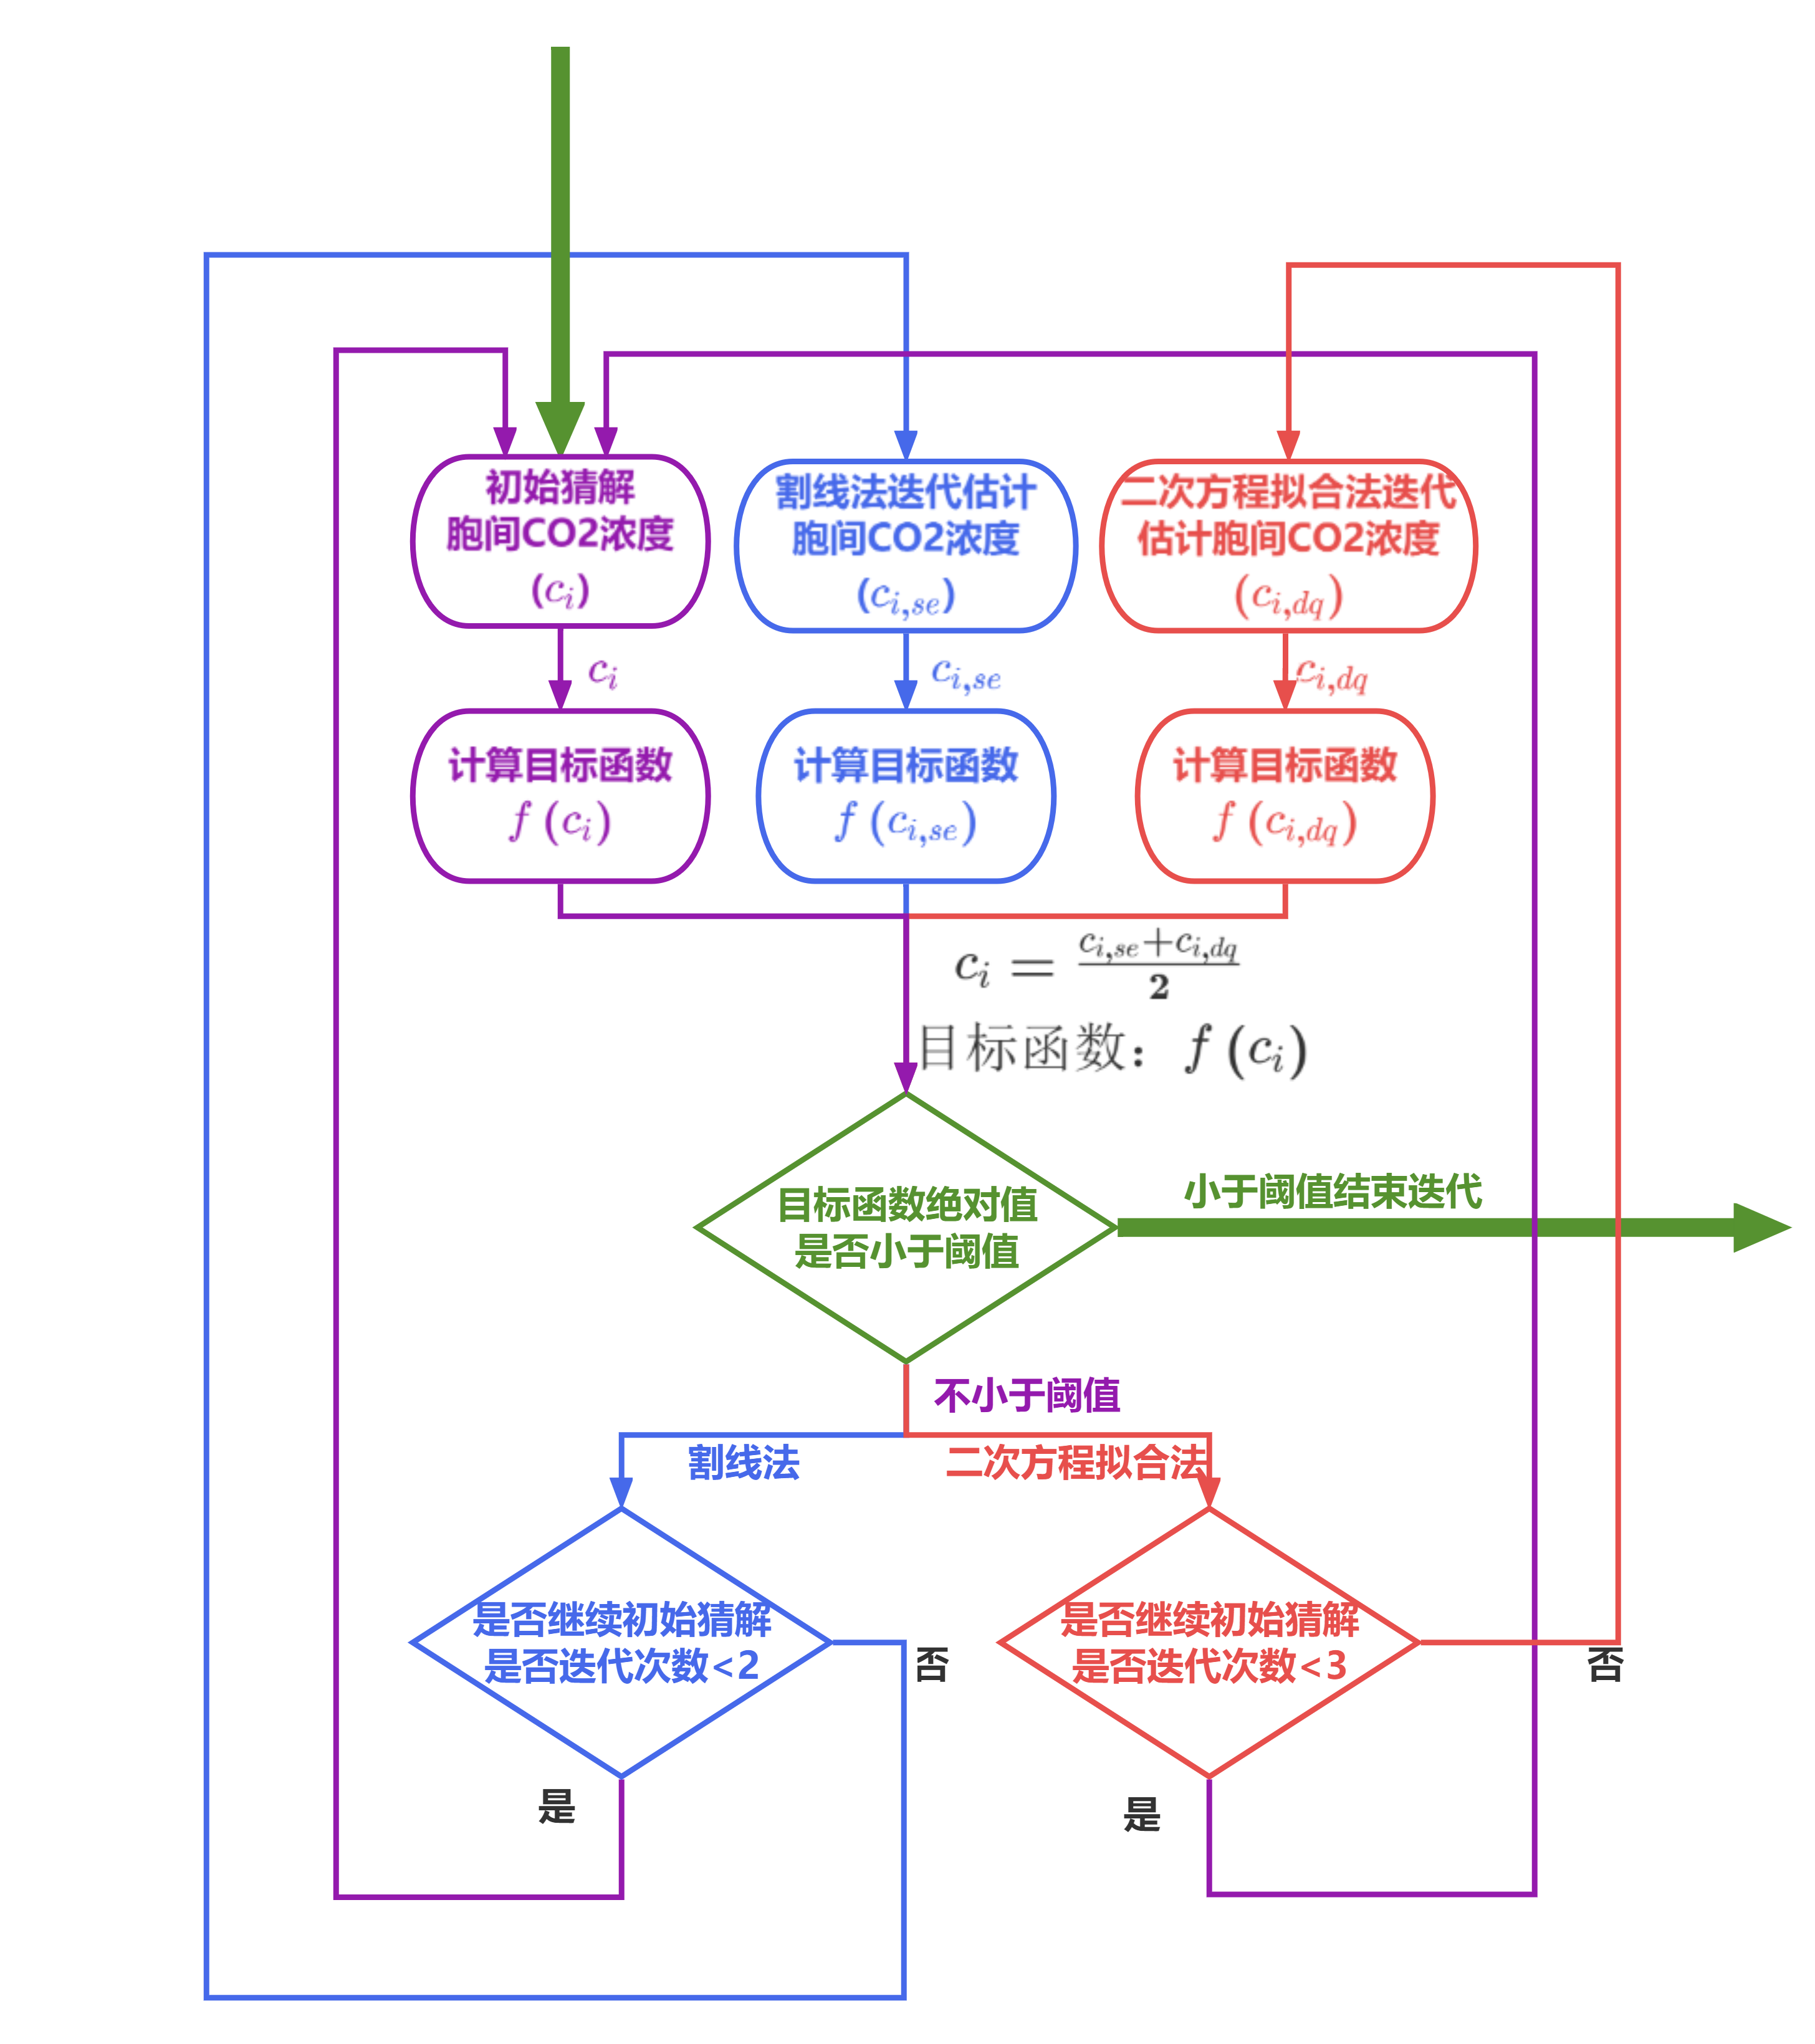
\includegraphics[width=0.9\textwidth]{Figures/气孔导度和光合作用/气孔数值解法流程图.png}
\caption{气孔数值解法流程图}
\label{fig:气孔数值解法流程图}
\end{figure}
}